
\section{Background \& Motivation}
Before proceeding, we first introduce notations used throughout this paper. $I$, $F$ and $O$ denote 4-dimension Input, Filter and Output
tensors respectively. And each tensor is indexed by $N$ (batch size), $C$ (channels), $H$ (height) and $W$ (width). For example, $I_N$,
$I_C$, $I_H$ and $I_W$ represent the batch size, the number of channels, width and height of the input.

The convolution operation is commonly used to extract various features from input feature maps via convolutional filters. The computation
in the convolution stage takes a batch of $I_N$ 2D multi-channel feature maps of size $I_C \times I_H \times I_W$ and a bank of $F_N$ 2D
multi-channel filters of size $F_C \times F_H \times F_W$ ($F_C = I_C$) as inputs. The result of convolution is a batch of $O_N$
($O_N=I_N$) 2D multi-channel output feature maps of size $O_C \times O_H \times O_W$ ($O_C=F_N$). To generate one output feature map, all
filters are used to convolve with the same input feature map. Each filter slides over the input feature map and performs an elementwise
multiplication with the part of input it is currently on, and then summing up the results over all channels.

\begin{figure}
\centering
  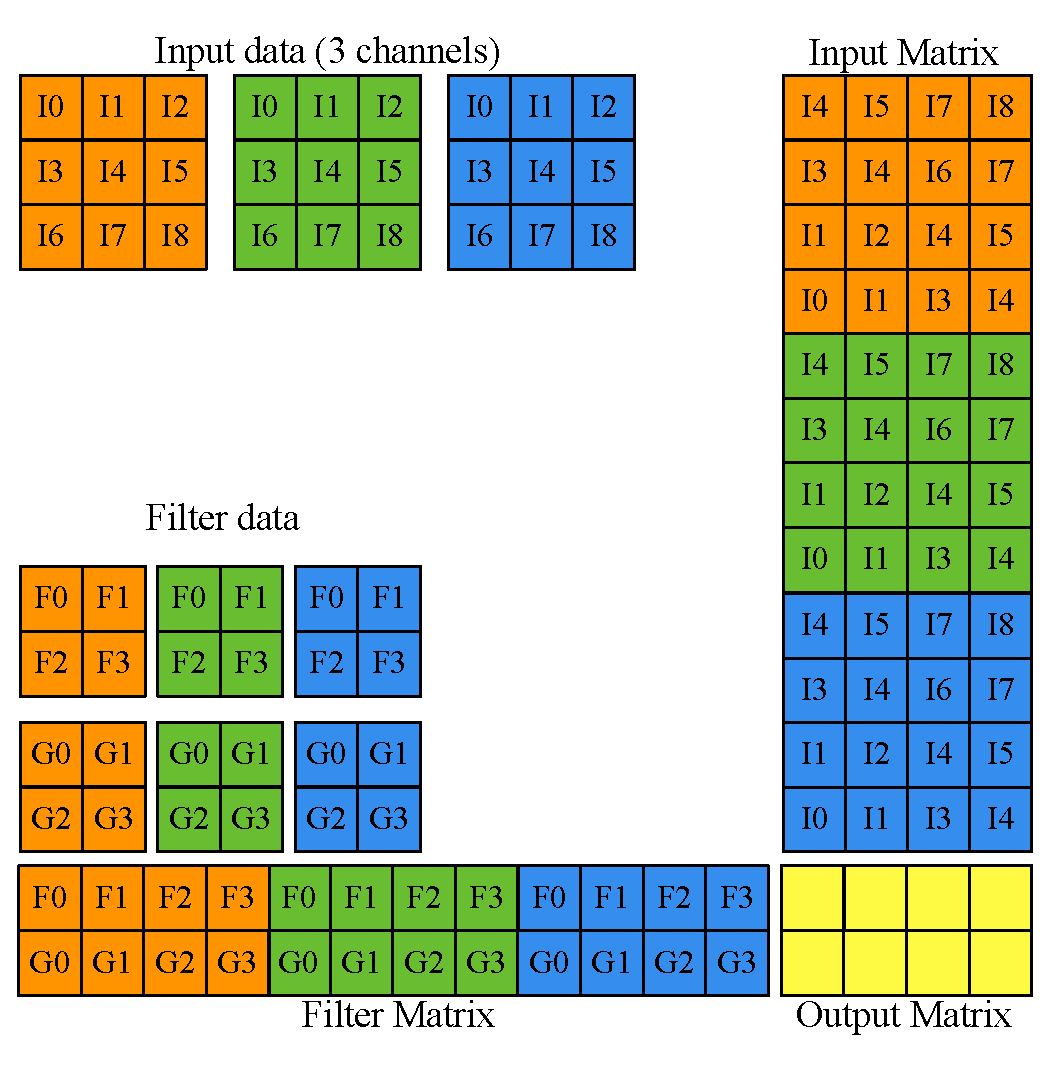
\includegraphics[width=0.75\columnwidth,height=6cm]{./figure/convlowering.eps}
  \caption{An illustration of how to convert a simple convolution into a matrix multiplication. Two filters are used to convolve with a 3-channel input.}
  \label{fig:convlowering}
\end{figure}

Many algorithms like FFT-based and Winograd-based convolutions have been proposed to optimize convolution operation, but they all need to
transform 4D tensors into the desired matrix, which incurs high memory overhead. Figure \ref{fig:convlowering}, which is taken from
\cite{ChetlurWVCTCS14}, illustrates how to convert a simple convolution into a matrix multiplication. We can see that there are many
duplicate elements in Input Matrix, which can increase the memory overhead and offset some performance gains brought by the reduction in
computation complexity.

We examine the process of convolution and propose two optimization algorithms to reduce memory overhead. We use a simple 2D convolution as
a motivating example to demonstrate how our algorithms work. Figure \ref{fig:twostrategies} illustrates a simple 2D convolution on GPU. We
slide a $5 \times 5$ filter over a $6 \times 11$ image to produce a $2 \times 7$ output. Each CUDA thread calculates one column of output.
Thread 0 and thread 1 demonstrate the process of sliding the filter along the width dimension. We can see that thread 0 and thread 1 load
two overlapped regions from the input image, which generates four duplicate columns. Thread 6 demonstrates the process of sliding the
filter along the height dimension. We can see that thread 6 loads two overlapped regions and generates four duplicate rows.

Our optimization algorithms can eliminate two types of duplication and thus reduce the number of memory transactions. (1) Column reuse
algorithm, we let each thread load the first and last columns it needs and retrieve rest columns from other threads through CUDA shuffle
instructions. The difference in the usage of CUDA shuffle instructions between our algorithms and the previous study
\cite{vasilache2014fast} will be detailed in section \ref{sec:strategies}. (2) Row reuse algorithm, we let each CUDA thread load overlapped
rows only once and multiply each row with multiple rows of a filter to calculate multiple output elements. A major performance issue
encountered in our implementation is that thread local arrays with dynamic indexing will be put into the local memory which has the same
access latency as the global memory. To solve this problem, we use $pack$ and $unpack$ instructions provided by CUDA PTX assembly language
to transform dynamic indexing into static indexing.

\begin{figure}
\centering
  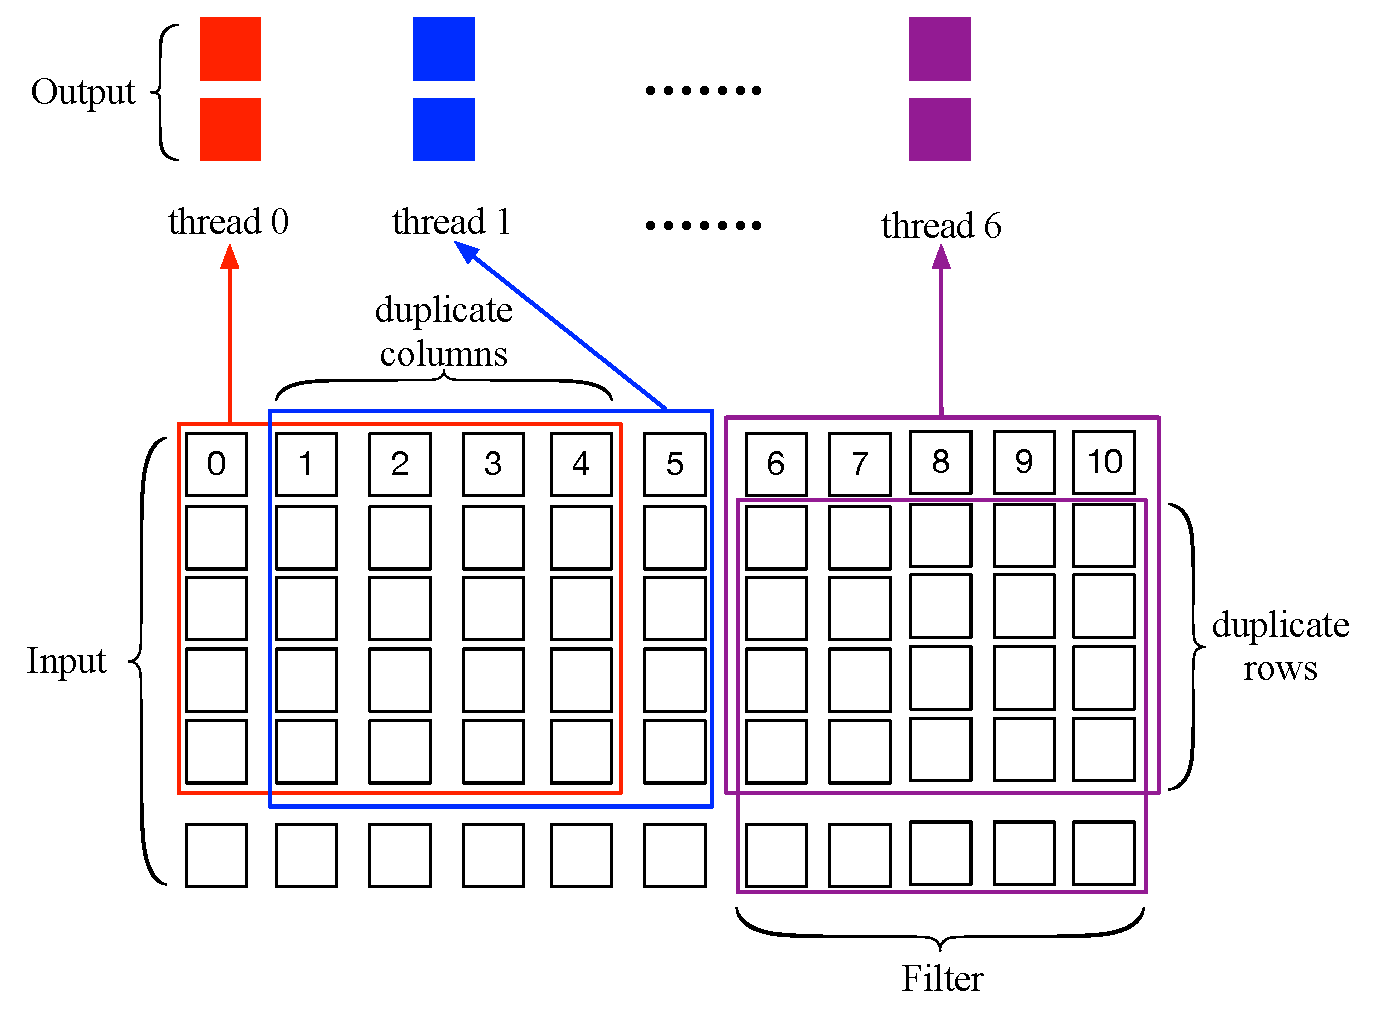
\includegraphics[width=\columnwidth,height=6cm]{./figure/twostrategies.eps}
  \caption{An illustration of how to perform 2D convolution on GPU. Filter size is $5 \times 5$, input image size is $6 \times 11$ and output size is $2 \times 7$. Each CUDA thread calculates one column of the output. Threads 0 and 1 load needed regions from input image with four duplicate columns. Thread 6 loads two overlapped regions from input image and generates four duplicate rows. Numbers in the square denote the index of input elements.}
  \label{fig:twostrategies}
\end{figure}
